\documentclass[11pt]{article}
\usepackage[preprint]{acl}
\usepackage{times}
\usepackage{latexsym}
\usepackage[T1]{fontenc}
\usepackage[utf8]{inputenc}
\usepackage{microtype}
\usepackage{inconsolata}
\usepackage{graphicx}
\usepackage{booktabs}
\usepackage{array}
\newcolumntype{L}[1]{>{\raggedright\arraybackslash}p{#1}}
\usepackage{amsmath}
\usepackage{textcomp}
\usepackage{CJKutf8}
\newcommand{\zh}[1]{\begin{CJK}{UTF8}{bsmi}#1\end{CJK}}
\usepackage{tikz}
\usetikzlibrary{positioning,arrows.meta}

% All numbers below come from generated/numbers.tex (src/07_paper_assets.py).
\newcommand{\abA}{0.367}
\newcommand{\abB}{0.349}
\newcommand{\abBplus}{0.347}
\newcommand{\abC}{0.328}
\newcommand{\abNoEdu}{0.345}
\newcommand{\abNoLevel}{0.483}
\newcommand{\abNoMom}{0.348}
\newcommand{\alphaSel}{0.001}
\newcommand{\bDfive}{0.205}
\newcommand{\bDfiveRaw}{0.53}
\newcommand{\bEdu}{\ensuremath{-}0.137}
\newcommand{\bEduX}{\ensuremath{-}0.212}
\newcommand{\bTfr}{1.423}
\newcommand{\birthsMedErr}{7.4}
\newcommand{\caseFive}{Egypt (TFR$_t$ 3.25, $\Delta_5$ \ensuremath{-}0.25, schooling 8.1 yr; actual 3.50, forecast 2.67, error +0.83)}
\newcommand{\caseFour}{Kyrgyzstan (TFR$_t$ 2.64, $\Delta_5$ +0.07, schooling 9.4 yr; actual 3.21, forecast 2.36, error +0.85)}
\newcommand{\caseOne}{Mongolia (TFR$_t$ 1.99, $\Delta_5$ \ensuremath{-}0.26, schooling 8.9 yr; actual 3.01, forecast 1.75, error +1.26)}
\newcommand{\caseThree}{the Central African Republic (TFR$_t$ 5.81, $\Delta_5$ \ensuremath{-}0.04, schooling 3.1 yr; actual 6.13, forecast 5.25, error +0.87)}
\newcommand{\caseTwo}{Zimbabwe (TFR$_t$ 3.69, $\Delta_5$ \ensuremath{-}0.32, schooling 8.5 yr; actual 3.91, forecast 2.93, error +0.99)}
\newcommand{\cvAdult}{0.331}
\newcommand{\cvAllGroups}{0.350}
\newcommand{\cvEduGainAbs}{0.017}
\newcommand{\cvEduGapAll}{\ensuremath{-}0.017}
\newcommand{\cvEduGapAllHi}{0.008}
\newcommand{\cvEduGapAllLo}{\ensuremath{-}0.040}
\newcommand{\cvEduGapHigh}{\ensuremath{-}0.032}
\newcommand{\cvEduGapHighHi}{0.015}
\newcommand{\cvEduGapHighLo}{\ensuremath{-}0.077}
\newcommand{\cvEduGapHighN}{265}
\newcommand{\cvGap}{0.327}
\newcommand{\cvGapBest}{\ensuremath{-}0.014}
\newcommand{\cvGapBestHi}{0.013}
\newcommand{\cvGapBestLo}{\ensuremath{-}0.040}
\newcommand{\cvHinge}{0.338}
\newcommand{\cvKnotFiveFive}{0.351}
\newcommand{\cvLasso}{0.328}
\newcommand{\cvMaeDamped}{0.425}
\newcommand{\cvMaeGbm}{0.347}
\newcommand{\cvMaeOurs}{0.328}
\newcommand{\cvMaePersist}{0.661}
\newcommand{\cvMaeRf}{0.354}
\newcommand{\cvMaeRfC}{0.342}
\newcommand{\cvMaeRidgeRaw}{0.367}
\newcommand{\cvMaeSingle}{0.807}
\newcommand{\cvOLS}{0.328}
\newcommand{\cvPairedP}{0.53}
\newcommand{\cvPairedT}{\ensuremath{-}0.71}
\newcommand{\cvSdDamped}{0.089}
\newcommand{\cvSdGbm}{0.044}
\newcommand{\cvSdOurs}{0.052}
\newcommand{\cvSdPersist}{0.102}
\newcommand{\cvSdRf}{0.040}
\newcommand{\cvSdRfC}{0.025}
\newcommand{\cvSdRidgeRaw}{0.068}
\newcommand{\cvSdSingle}{0.034}
\newcommand{\dampedPhi}{0.6}
\newcommand{\eaChnE}{\ensuremath{-}0.45}
\newcommand{\eaChnP}{1.68}
\newcommand{\eaChnY}{1.24}
\newcommand{\eaKorE}{\ensuremath{-}0.42}
\newcommand{\eaKorP}{1.23}
\newcommand{\eaKorY}{0.81}
\newcommand{\eaTwnE}{+0.14}
\newcommand{\eaTwnFifteenP}{0.96}
\newcommand{\eaTwnFifteenY}{1.18}
\newcommand{\eaTwnP}{0.85}
\newcommand{\eaTwnY}{0.99}
\newcommand{\eduGainHi}{0.013}
\newcommand{\eduGainLo}{0.004}
\newcommand{\effFive}{\ensuremath{-}0.087}
\newcommand{\effFiveHi}{\ensuremath{-}0.059}
\newcommand{\effFiveLo}{\ensuremath{-}0.115}
\newcommand{\effSeven}{\ensuremath{-}0.179}
\newcommand{\effSevenHi}{\ensuremath{-}0.117}
\newcommand{\effSevenLo}{\ensuremath{-}0.241}
\newcommand{\effThreeHigh}{0.54}
\newcommand{\effThreeLow}{0.12}
\newcommand{\effTwo}{\ensuremath{-}0.041}
\newcommand{\effTwoHi}{\ensuremath{-}0.018}
\newcommand{\effTwoLo}{\ensuremath{-}0.064}
\newcommand{\foldMaxRows}{1015}
\newcommand{\foldMinRows}{580}
\newcommand{\gapCvsA}{\ensuremath{-}0.039}
\newcommand{\gapCvsAHi}{\ensuremath{-}0.007}
\newcommand{\gapCvsALo}{\ensuremath{-}0.071}
\newcommand{\gapCvsB}{\ensuremath{-}0.021}
\newcommand{\gapCvsBHi}{0.008}
\newcommand{\gapCvsBLo}{\ensuremath{-}0.047}
\newcommand{\gapDamped}{\ensuremath{-}0.079}
\newcommand{\gapDampedAbs}{0.079}
\newcommand{\gapDampedHi}{\ensuremath{-}0.051}
\newcommand{\gapDampedLo}{\ensuremath{-}0.107}
\newcommand{\gapGbm}{\ensuremath{-}0.049}
\newcommand{\gapGbmAbs}{0.049}
\newcommand{\gapGbmHi}{\ensuremath{-}0.025}
\newcommand{\gapGbmLo}{\ensuremath{-}0.073}
\newcommand{\gapRf}{\ensuremath{-}0.052}
\newcommand{\gapRfC}{\ensuremath{-}0.036}
\newcommand{\gapRfCHi}{\ensuremath{-}0.016}
\newcommand{\gapRfCLo}{\ensuremath{-}0.058}
\newcommand{\gapRfHi}{\ensuremath{-}0.028}
\newcommand{\gapRfLo}{\ensuremath{-}0.079}
\newcommand{\gapRidgeRaw}{\ensuremath{-}0.054}
\newcommand{\gapRidgeRawHi}{\ensuremath{-}0.026}
\newcommand{\gapRidgeRawLo}{\ensuremath{-}0.082}
\newcommand{\gdpMissing}{20}
\newcommand{\knot}{4}
\newcommand{\lagOld}{\ensuremath{-}0.07}
\newcommand{\lagYoung}{\ensuremath{-}0.33}
\newcommand{\lorMaxDiff}{0.025}
\newcommand{\lorSsaIn}{0.317}
\newcommand{\lorSsaOut}{0.342}
\newcommand{\miEdu}{0.61}
\newcommand{\miTfr}{1.25}
\newcommand{\minPred}{0.85}
\newcommand{\nCountries}{145}
\newcommand{\nFeatures}{5}
\newcommand{\olsRsq}{0.94}
\newcommand{\pCvsA}{0.08}
\newcommand{\pCvsB}{0.22}
\newcommand{\partialEduAll}{\ensuremath{-}0.09}
\newcommand{\partialEduGdpQ}{\ensuremath{-}0.33}
\newcommand{\partialEduTfr}{\ensuremath{-}0.34}
\newcommand{\partialGap}{0.05}
\newcommand{\partialQfiveTfr}{0.44}
\newcommand{\piCov}{88}
\newcommand{\piCovHigh}{80}
\newcommand{\piWidthHigh}{1.21}
\newcommand{\piWidthLow}{0.83}
\newcommand{\rDfiveDy}{0.40}
\newcommand{\rDfiveY}{0.30}
\newcommand{\rEduY}{\ensuremath{-}0.85}
\newcommand{\rFemMale}{0.96}
\newcommand{\rTfrQfive}{0.89}
\newcommand{\rTfrY}{0.95}
\newcommand{\revAll}{0.21}
\newcommand{\revHigh}{0.47}
\newcommand{\revLow}{0.11}
\newcommand{\rhoEduY}{\ensuremath{-}0.84}
\newcommand{\ridgeCiDiff}{0.01}
\newcommand{\rowsGap}{145}
\newcommand{\rowsTest}{290}
\newcommand{\rowsTrain}{1305}
\newcommand{\scenAvg}{50}
\newcommand{\scenMed}{47}
\newcommand{\scenP}{0.72}
\newcommand{\scenRev}{63}
\newcommand{\scenRt}{48}
\newcommand{\slAdvC}{0.144}
\newcommand{\slCLow}{0.173}
\newcommand{\slCMid}{0.252}
\newcommand{\slCOnset}{0.315}
\newcommand{\slCPre}{0.325}
\newcommand{\slGbmLow}{0.185}
\newcommand{\slGbmMid}{0.315}
\newcommand{\slGbmOnset}{0.503}
\newcommand{\slGbmPre}{0.362}
\newcommand{\slMenaBias}{+0.17}
\newcommand{\slMenaC}{0.288}
\newcommand{\slNLow}{154}
\newcommand{\slNMid}{75}
\newcommand{\slNOnset}{35}
\newcommand{\slNPre}{26}
\newcommand{\slNoEduLow}{0.205}
\newcommand{\slNoEduMid}{0.208}
\newcommand{\slNoEduOnset}{0.269}
\newcommand{\slNoEduPre}{0.360}
\newcommand{\slSsaBias}{+0.13}
\newcommand{\slSsaC}{0.317}
\newcommand{\slopeNineties}{\ensuremath{-}0.025}
\newcommand{\slopeSixties}{\ensuremath{-}0.170}
\newcommand{\stageLowR}{\ensuremath{-}0.18}
\newcommand{\stageMidR}{\ensuremath{-}0.19}
\newcommand{\stagePreHi}{\ensuremath{-}0.38}
\newcommand{\stagePreLo}{\ensuremath{-}0.59}
\newcommand{\stagePreN}{566}
\newcommand{\stagePreR}{\ensuremath{-}0.48}
\newcommand{\teA}{0.278}
\newcommand{\teB}{0.247}
\newcommand{\teBiasYearA}{+0.15}
\newcommand{\teBiasYearB}{\ensuremath{-}0.02}
\newcommand{\teEduGapAll}{\ensuremath{-}0.004}
\newcommand{\teEduGapAllHi}{0.015}
\newcommand{\teEduGapAllLo}{\ensuremath{-}0.021}
\newcommand{\teEduGapAllN}{290}
\newcommand{\teEduGapHigh}{0.011}
\newcommand{\teEduGapHighHi}{0.082}
\newcommand{\teEduGapHighLo}{\ensuremath{-}0.054}
\newcommand{\teEduGapHighN}{61}
\newcommand{\teEduGapLow}{\ensuremath{-}0.008}
\newcommand{\teEduGapLowHi}{0.007}
\newcommand{\teEduGapLowLo}{\ensuremath{-}0.021}
\newcommand{\teEduGapLowN}{229}
\newcommand{\teHinge}{0.237}
\newcommand{\teHingeGapAll}{\ensuremath{-}0.013}
\newcommand{\teHingeGapAllHi}{0.000}
\newcommand{\teHingeGapAllLo}{\ensuremath{-}0.027}
\newcommand{\teHingeGapHigh}{\ensuremath{-}0.013}
\newcommand{\teHingeGapHighHi}{0.036}
\newcommand{\teHingeGapHighLo}{\ensuremath{-}0.062}
\newcommand{\teHingeGapLow}{\ensuremath{-}0.013}
\newcommand{\teHingeGapLowHi}{\ensuremath{-}0.002}
\newcommand{\teHingeGapLowLo}{\ensuremath{-}0.024}
\newcommand{\teHitDamped}{40}
\newcommand{\teHitGbm}{49}
\newcommand{\teHitOurs}{56}
\newcommand{\teHitPersist}{37}
\newcommand{\teHitRf}{50}
\newcommand{\teHitRfC}{49}
\newcommand{\teHitRidgeRaw}{47}
\newcommand{\teHitSingle}{19}
\newcommand{\teMaeDamped}{0.303}
\newcommand{\teMaeGbm}{0.273}
\newcommand{\teMaeHi}{0.250}
\newcommand{\teMaeLo}{0.200}
\newcommand{\teMaeOurs}{0.224}
\newcommand{\teMaePersist}{0.378}
\newcommand{\teMaeRf}{0.276}
\newcommand{\teMaeRfC}{0.260}
\newcommand{\teMaeRidgeRaw}{0.278}
\newcommand{\teMaeSingle}{0.657}
\newcommand{\teMaeYearA}{0.241}
\newcommand{\teMaeYearB}{0.207}
\newcommand{\teNoEdu}{0.228}
\newcommand{\teRmseDamped}{0.395}
\newcommand{\teRmseGbm}{0.377}
\newcommand{\teRmseOurs}{0.300}
\newcommand{\teRmsePersist}{0.497}
\newcommand{\teRmseRf}{0.386}
\newcommand{\teRmseRfC}{0.346}
\newcommand{\teRmseRidgeRaw}{0.361}
\newcommand{\teRmseSingle}{0.820}
\newcommand{\teRsqDamped}{0.91}
\newcommand{\teRsqGbm}{0.92}
\newcommand{\teRsqOurs}{0.95}
\newcommand{\teRsqPersist}{0.85}
\newcommand{\teRsqRf}{0.91}
\newcommand{\teRsqRfC}{0.93}
\newcommand{\teRsqRidgeRaw}{0.92}
\newcommand{\teRsqSingle}{0.60}
\newcommand{\thrExcess}{0.024}
\newcommand{\threshold}{0.2}
\newcommand{\tuneMax}{0.621}
\newcommand{\tuneOne}{0.329}
\newcommand{\twBirths}{161}
\newcommand{\twBirthsErr}{22}
\newcommand{\twHi}{1.26}
\newcommand{\twLo}{0.43}
\newcommand{\twUn}{1.13}
\newcommand{\twnSixty}{5.8}
\newcommand{\twnTwentyThree}{0.87}
\newcommand{\unAvgGap}{\ensuremath{-}0.016}
\newcommand{\unAvgGapHi}{\ensuremath{-}0.005}
\newcommand{\unAvgGapLo}{\ensuremath{-}0.027}
\newcommand{\unGapA}{0.029}
\newcommand{\unGapAHi}{0.058}
\newcommand{\unGapALo}{0.001}
\newcommand{\unGapAll}{\ensuremath{-}0.006}
\newcommand{\unGapAllHi}{0.016}
\newcommand{\unGapAllLo}{\ensuremath{-}0.027}
\newcommand{\unGapB}{\ensuremath{-}0.040}
\newcommand{\unGapBHi}{\ensuremath{-}0.012}
\newcommand{\unGapBLo}{\ensuremath{-}0.071}
\newcommand{\unHighRev}{0.326}
\newcommand{\unHighRt}{0.656}
\newcommand{\unHighUn}{0.720}
\newcommand{\unMaeAAvg}{0.314}
\newcommand{\unMaeARev}{0.242}
\newcommand{\unMaeARt}{0.342}
\newcommand{\unMaeAUn}{0.313}
\newcommand{\unMaeAvg}{0.328}
\newcommand{\unMaeBAvg}{0.342}
\newcommand{\unMaeBRev}{0.208}
\newcommand{\unMaeBRt}{0.335}
\newcommand{\unMaeBUn}{0.375}
\newcommand{\unMaeRev}{0.225}
\newcommand{\unMaeRt}{0.338}
\newcommand{\unMaeUn}{0.344}
\newcommand{\unN}{287}
\newcommand{\vifEduMax}{32}
\newcommand{\vifMax}{16}
\newcommand{\vifStage}{12}
\newcommand{\vifTfr}{16}
\newcommand{\yMax}{8.86}
\newcommand{\yMin}{0.81}

% \input is not expandable inside tabular; use the TeX primitive for generated table bodies.
\makeatletter\newcommand{\tabinput}[1]{\@@input #1 }\makeatother

% ---------------------------------------------------------------- TEAM: fill these in
\newcommand{\teamid}{13}
\newcommand{\repourl}{\url{https://github.com/franbrizuelab/nycu-dm-hw1-fertility}}

\title{Does Women's Schooling Today Improve a Ten-Year Fertility Forecast?\\A Leak-Free Linear Benchmark for 145 Countries}

\author{Team \teamid{} \\
  \zh{李尚哲} \quad \zh{呂丞頤} \quad \zh{黃駿甯} \quad \zh{吳美真} \\
  \zh{孫傅康} \quad \zh{傅維雨} \quad \zh{張凱華} \quad \zh{李玠廷} \\
  National Yang Ming Chiao Tung University \\
  GitHub: \repourl}

\begin{document}
\maketitle

\begin{abstract}
Planners who size school intakes and pension systems need each country's fertility a decade ahead. We ask how much women's schooling adds to a ten-year forecast of the total fertility rate (TFR) beyond fertility's own trajectory. Using UN and Barro--Lee data for \nCountries{} countries and a rolling-origin protocol with a ten-year embargo, a \nFeatures{}-feature ridge model reaches a test MAE of \teMaeOurs{} children per woman for 2015 and 2020, ahead of gradient boosting and a damped-trend rule. Fed only the data available at the time, it matches the UN's own projections (\unMaeRt{} vs.\ \unMaeUn), and averaging the two lowers error significantly. Schooling has a significant, stage-dependent coefficient but improves out-of-sample MAE by only \eduGainLo--\eduGainHi. For planners, the larger lesson is that later revisions of \emph{current} fertility (\revAll{} on average) are as large as ten-year forecast errors.
\end{abstract}

% ======================================================================
\section{Introduction}
Taiwan's TFR fell from \twnSixty{} in 1960 to \twnTwentyThree{} in 2023 \citep{un2024wpp}; school and pension plans commit resources a decade ahead. Planners default to the UN \emph{World Population Prospects} (WPP), whose high and low variants sit $\pm$0.4 children per woman around the medium variant in years 6--10 of a projection \citep{un2024methodology}. \textbf{The decision we support} is which of these scenarios to plan for: a ten-year forecast with an error below 0.2, half that spacing, tells the planner which scenario their country is on.

Women's education is the most cited driver of fertility decline \citep{lutz2011global,bongaarts2003completing}, and education now drives global fertility forecasts \citep{vollset2020fertility}. \textbf{Research question:} \emph{How much does women's schooling at year $t$ improve a linear forecast of TFR at $t{+}10$ beyond fertility's own trajectory, and for which countries?}

\textbf{Contributions.} (C1) A leak-free ten-year TFR benchmark on which a \nFeatures{}-feature linear model beats tree ensembles and a damped-trend rule (\S\ref{sec:main}). (C2) Ablation evidence that fertility's level and momentum carry most of the skill, and that our engineered set beats both the raw columns and a correlation-ranked set (\S\ref{sec:ablation}). (C3) Education's coefficient is stage-dependent and significant in sample (\S\ref{sec:coef}), but its out-of-sample gain is small and not significant. (C4) A real-time benchmark against the UN's own projections and the planner's scenario decision, with errors in births (\S\ref{sec:practical}).

% ======================================================================
\section{Related Work}
The UN's Bayesian hierarchical model \citep{alkema2011probabilistic,raftery2014bayesian} projects TFR from each country's own history plus the pooled shape of the transition, with no education input. Projected from a 1990--95 base, its median had mean squared errors of 0.17 for 2000--05 and 0.21 for 2005--10 (RMSE 0.41--0.46; ours: \teRmseOurs{} for 2015/2020). IHME \citep{vollset2020fertility} instead models completed cohort fertility as a function of female educational attainment and contraceptive met need, and reports scenario uncertainty rather than a held-out error. At the micro level, \citet{kebede2019stalls} trace the stalled African fertility declines of the 2000s to education disruptions of the 1980s, and \citet{adhikari2024forecasting} forecast African fertility by education group from 138 DHS surveys and validate on later birth cohorts. \textbf{Our difference:} we test schooling as a \emph{forecasting input} under strict time ordering, against fertility-only baselines that share the same folds. We measure its incremental value, not its association, and score it against the UN projections planners actually used.


% ======================================================================
\section{Task Definition and Data}
\label{sec:data}
\textbf{Task card.} \emph{Target:} the period TFR of a country in year $t{+}10$, in children per woman (observed range \yMin--\yMax). \emph{One row:} a country at start year $t\in\{1955,1960,\dots,2010\}$. \emph{Inputs:} only values dated $t$ or earlier: TFR$_t$ and TFR$_{t-5}$, under-5 mortality, years of schooling by sex and age band, GDP per capita, urban share and region. \emph{Prediction time:} year $t$.

\textbf{Sources.} TFR and under-5 mortality come from WPP 2024, which has observed estimates through 2023 \citep{un2024wpp}. Schooling comes from Barro--Lee v3 (sex $\times$ 10-year age band, 1950--2015) \citep{barro2013new}. The older v2.2, with 5-year bands, is used only in \S\ref{sec:eda}. GDP per capita comes from Penn World Table 10.01 \citep{feenstra2015next} and urban share from WUP 2025 \citep{un2025wup}. All are public and include Taiwan (World Bank data do not); files are downloaded by script with SHA-256 checksums, and an ISO3 join gives \nCountries{} countries.

\textbf{Preprocessing and why.} (i) Targets stop at 2020, because WPP values after 2023 are projections, and a projected target would leak the UN's model into ours. (ii) Rows with $t{=}2000$ are embargoed (\S\ref{sec:setup}). (iii) GDP is missing for \gdpMissing\% of training rows, mostly in the 1950s--60s. We impute the training-fold median with a missing indicator inside each fold, because dropping these rows would remove early Africa. (iv) Mortality and GDP are logged (right-skewed, Table~\ref{tab:summary}); (v) features are standardized in the pipeline; (vi) extremes are real, so nothing is clipped. The panel has \rowsTrain{} training rows ($t\le1995$), \rowsTest{} test rows ($t\in\{2005,2010\}$) and \rowsGap{} embargoed rows.

\begin{table}[t]
\centering\scriptsize
\setlength{\tabcolsep}{3pt}
\begin{tabular}{@{}lrrrrr@{}}
\toprule
Variable & Mean & SD & Min & Max & Miss.\% \\
\midrule
\tabinput{generated/tab_summary.tex}
\bottomrule
\end{tabular}
\caption{Training rows ($t\le1995$, n=\rowsTrain). TFR in children per woman. $\Delta_5$TFR$_t=\mathrm{TFR}_t-\mathrm{TFR}_{t-5}$.}
\label{tab:summary}
\end{table}

% ======================================================================
\section{Exploratory Feature Analysis}
\label{sec:eda}
All statistics in this section use training rows only (Fig.~\ref{fig:eda}).

\begin{figure*}[t]
\centering
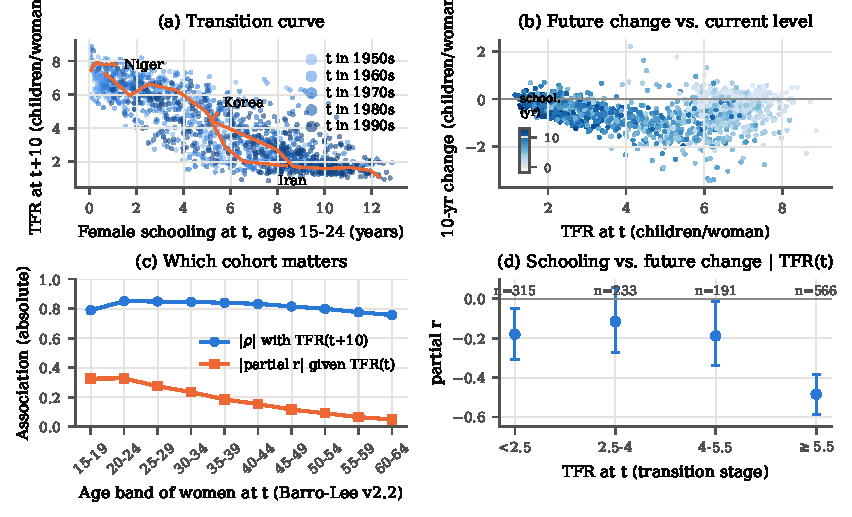
\includegraphics[width=0.74\textwidth]{../results/figures/fig_eda.pdf}
\caption{Exploration on training rows. (a) Future TFR against young women's schooling, with three country paths. (b) The 10-year change is largest in mid-transition. (c) Cohort lag curve: the schooling of women aged 15--24 at $t$ carries the most information beyond TFR$_t$. (d) Partial correlation of schooling with the future change, given TFR$_t$, by stage. Bars: 95\% CIs from a country-cluster bootstrap.}
\label{fig:eda}
\end{figure*}

\textbf{H1 (transition curve).} Young women's schooling tracks future TFR closely (Pearson $r{=}\rEduY$, Spearman $\rho{=}\rhoEduY$; Fig.~\ref{fig:eda}a), but current TFR tracks it more closely still ($r{=}\rTfrY$). Given TFR$_t$ and TFR$_t^2$, schooling's partial $r$ drops to \partialEduTfr. \emph{Decision:} test schooling as an increment on fertility's own level.
\textbf{H2 (which cohort).} With Barro--Lee v2.2's 5-year bands, the partial $r$ with TFR$_{t+10}$ given TFR$_t$ peaks at ages 20--24 (\lagYoung) and fades to \lagOld{} at 55--59 (Fig.~\ref{fig:eda}c). They are 25--34, peak childbearing ages, at $t{+}10$. \emph{Decision:} use schooling of women 15--24.
\textbf{H3 (redundancy).} Female and male schooling are nearly collinear ($r{=}\rFemMale$, VIF up to \vifEduMax), and the gender gap adds nothing given average schooling and TFR (partial $r{=}\partialGap$). \emph{Decision:} drop male schooling and the gap. H3 is rejected.
\textbf{H4 (confounding).} Controlling for log GDP and log mortality, schooling keeps a partial $r$ of \partialEduGdpQ. Adding TFR$_t$, TFR$_t^2$ and $\Delta_5$ shrinks it to \partialEduAll: schooling's information overlaps with the trajectory.
\textbf{H5 (stage).} Decline is fastest in mid-transition (Fig.~\ref{fig:eda}b). At TFR$_t\geq5.5$, schooling's partial $r$ with the future change is \stagePreR{} [\stagePreLo, \stagePreHi], against \stageMidR{} to \stageLowR{} at lower stages (Fig.~\ref{fig:eda}d). \emph{Decision:} gate schooling by stage.
\textbf{H6 (momentum).} The last five-year change correlates with the next ten-year change ($r{=}\rDfiveDy$). \emph{Decision:} add $\Delta_5$.
\textbf{H7 (stability).} The schooling slope given TFR$_t$ shrinks from \slopeSixties{} (1960s) to \slopeNineties{} (1990s). Fewer countries remain pre-transition over time, so this drift fits H5 (revisited in \S\ref{sec:errors}). A Pearson/Spearman/MI table (repository) ranks Set~B.

% ======================================================================
\section{Method}
\label{sec:method}
\begin{figure}[t]
\centering
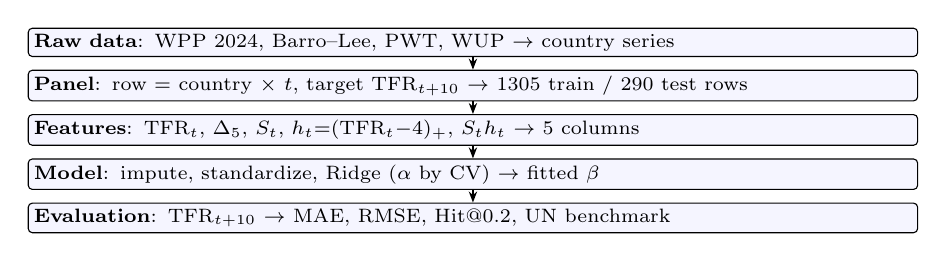
\begin{tikzpicture}[node distance=1.6mm, every node/.style={font=\scriptsize},
  box/.style={draw, rounded corners=1.5pt, align=left, text width=0.92\columnwidth, inner sep=2pt, fill=blue!4},
  arr/.style={-{Stealth[length=1.4mm]}, thick}]
\node[box] (raw) {\textbf{Raw data}: WPP 2024, Barro--Lee, PWT, WUP $\rightarrow$ country series};
\node[box, below=of raw] (panel) {\textbf{Panel}: row = country $\times$ $t$, target TFR$_{t+10}$ $\rightarrow$ \rowsTrain{} train / \rowsTest{} test rows};
\node[box, below=of panel] (feat) {\textbf{Features}: TFR$_t$, $\Delta_5$, $S_t$, $h_t{=}(\mathrm{TFR}_t{-}\knot)_+$, $S_t h_t$ $\rightarrow$ \nFeatures{} columns};
\node[box, below=of feat] (model) {\textbf{Model}: impute, standardize, Ridge ($\alpha$ by CV) $\rightarrow$ fitted $\beta$};
\node[box, below=of model] (eval) {\textbf{Evaluation}: TFR$_{t+10}$ $\rightarrow$ MAE, RMSE, Hit@0.2, UN benchmark};
\foreach \a/\b in {raw/panel, panel/feat, feat/model, model/eval} \draw[arr] (\a) -- (\b);
\end{tikzpicture}
\caption{Pipeline, input $\rightarrow$ output per stage. Imputation, scaling and model are fitted inside each training fold.}
\label{fig:pipeline}
\end{figure}

\textbf{Feature groups} (Fig.~\ref{fig:pipeline}). \emph{Level}: TFR$_t$. \emph{Momentum} (a lag feature, H6): $\Delta_5$TFR$_t$, the pace of an ongoing decline. \emph{Education stage} (domain-derived, H2/H5): $S_t$, the hinge $h_t=\max(0,\mathrm{TFR}_t-\kappa)$ and the interaction $S_t h_t$. Schooling gets an extra slope while fertility is high. The knot was set a priori at 5.5 (Fig.~\ref{fig:eda}d) and tuned over $\{4,4.5,\dots,6\}$ by CV, which picked $\kappa{=}\knot$ (CV MAE \abC{} vs.\ \cvKnotFiveFive{} at 5.5). \emph{Curvature} (TFR$_t^2$, Fig.~\ref{fig:eda}b), \emph{development} (log mortality, log GDP, urban share; H4) and \emph{region} dummies were also candidates. Backward group elimination on CV removed development, then region, then curvature, and lowered CV MAE from \cvAllGroups{} to \abC.

\textbf{Model choice and tuning.} The hinge is a function of TFR$_t$, so the two are collinear by construction (VIF up to \vifMax; Table~\ref{tab:coef}). Ridge stabilizes both without discarding either. We search 13 log-spaced values of $\alpha\in[10^{-3},10^{3}]$ on the folds of \S\ref{sec:setup}, minimizing mean fold MAE. CV MAE is flat (\abC--\tuneOne) for $\alpha\le1$ and rises to \tuneMax{} at $10^3$, so CV selects $\alpha{=}\alphaSel$. With \nFeatures{} features and \rowsTrain{} rows the penalty barely binds: OLS, Lasso and Elastic Net all reach \cvOLS. \S\ref{sec:coef} therefore reports OLS. Predictions are not clipped (minimum \minPred).

% ======================================================================
\section{Experimental Setup}
\label{sec:setup}
\textbf{Validation: a planner standing in year $v$.} A row with start year $t$ reveals TFR$_{t+10}$, so a planner at year $v$ may train only on rows with $t+10\le v$. Shuffled K-fold and row-based \texttt{TimeSeriesSplit} violate this ten-year embargo. We use four rolling-origin folds that validate at $v\in\{1980,\dots,1995\}$ and train on $t\le v-10$ (\foldMinRows--\foldMaxRows{} rows). Each fold is a full cross-section; 5-year data allow only four. Saved fold keys are reused by every method; we report mean $\pm$ SD over folds. \emph{Test:} the frozen design is refit on all $t\le1995$ rows and scored once on $t\in\{2005,2010\}$ (targets 2015, 2020). A hash lock stops re-scoring after any design change. GroupKFold is not used, since planners forecast known countries; leave-one-region-out is a robustness check. \emph{Disclosure:} while checking coverage we saw baseline-only test statistics; no model saw test data before the freeze.

\textbf{Metrics and threshold.} MAE (children per woman) is the typical miss. RMSE stresses large misses (schools built for a rebound that never comes). R$^2$ is context only. Hit@0.2 is the share of country-years forecast within 0.2. \textbf{Decision threshold: MAE $\le$ \threshold.} WPP's high and low variants sit $\pm$0.4 from the medium variant at this horizon \citep{un2024methodology}, so an error below the midpoint identifies the right scenario.

\textbf{Baselines.} In increasing strength: the training mean; persistence (TFR$_{t+10}{=}$TFR$_t$); a damped trend TFR$_t+2\phi\Delta_5$ with $\phi{=}\dampedPhi$ tuned by CV; single-feature OLS on schooling; random forest and gradient boosting on the raw columns, with grids tuned on the same folds; ridge on the raw columns; and a random forest on our features. Tools: scikit-learn \citep{pedregosa2011scikit}, statsmodels \citep{seabold2010statsmodels}. \textbf{Significance:} paired $t$-test over fold MAEs and a country-cluster bootstrap (2,000 resamples) of MAE gaps.

% ======================================================================
\section{Results}
\subsection{Main results}
\label{sec:main}
\begin{table}[t]
\centering\scriptsize
\setlength{\tabcolsep}{2.4pt}
\begin{tabular}{@{}lrrrrr@{}}
\toprule
& CV & \multicolumn{4}{c}{Test (targets 2015, 2020)} \\
\cmidrule(l){3-6}
Method & MAE{\tiny$\pm$SD} & MAE & RMSE & R$^2$ & Hit \\
\midrule
\tabinput{generated/tab_main.tex}
\bottomrule
\end{tabular}
\caption{Main results in children per woman. CV: mean$\pm$SD over 4 folds. Hit: share of test rows with $|$error$|<0.2$. Bold: best per column.}
\label{tab:main}
\end{table}

\textbf{Overall.} Our model has the lowest CV MAE (\cvMaeOurs{} $\pm$ \cvSdOurs) and the lowest test MAE: \teMaeOurs{}, 95\% CI [\teMaeLo, \teMaeHi] (Table~\ref{tab:main}). It forecasts \teHitOurs\% of country-years within 0.2. \textbf{Threshold:} the MAE exceeds \threshold{} by \thrExcess{} (the CI only touches it); \S\ref{sec:practical} tests the scenario decision directly. \textbf{Against the strongest baselines,} the test MAE gaps (ours $-$ baseline, country-cluster bootstrap CI) are \gapGbm{} [\gapGbmLo, \gapGbmHi] vs.\ gradient boosting, \gapRfC{} [\gapRfCLo, \gapRfCHi] vs.\ a random forest on the same features and \gapDamped{} [\gapDampedLo, \gapDampedHi] vs.\ the damped trend. In CV, the gap to the best baseline (random forest on our features) is not significant (paired $t$, $p{=}\cvPairedP$; pooled \cvGapBest{} [\cvGapBestLo, \cvGapBestHi]). We therefore claim a consistent edge, not a decisive win. \textbf{Why it wins:} trees predict piecewise constants learned on high-fertility 1955--95 data, while ridge extrapolates level plus momentum smoothly. The gap is widest at TFR$_t\in[\knot,5.5)$: \slCOnset{} for ours against \slGbmOnset{} for gradient boosting (Fig.~\ref{fig:test}b). Test errors are lower than CV errors for all methods because 2005--20 changes were smaller.

\begin{figure*}[t]
\centering
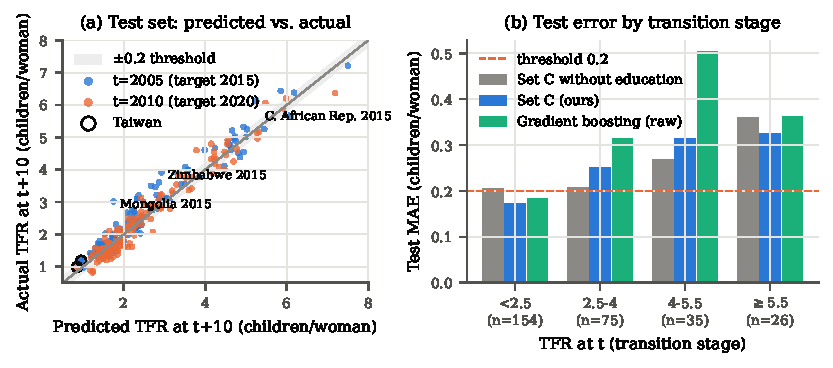
\includegraphics[width=0.74\textwidth]{../results/figures/fig_test.pdf}
\caption{Test set, scored once. (a) Predicted vs.\ actual TFR$_{t+10}$, with a $\pm$0.2 band. The three largest errors are labelled and Taiwan is circled. (b) Test MAE by transition stage: ours, ours without the education group, and gradient boosting on raw inputs.}
\label{fig:test}
\end{figure*}

\subsection{Feature ablation}
\label{sec:ablation}
\begin{table}[t]
\centering\scriptsize
\setlength{\tabcolsep}{2.2pt}
\begin{tabular}{@{}lrrrrrr@{}}
\toprule
& CV MAE & \multicolumn{4}{c}{Fold MAE (validation $t$)} & Test \\
\cmidrule(lr){3-6}
Feature set & {\tiny$\pm$SD} & 1980 & 1985 & 1990 & 1995 & MAE \\
\midrule
\tabinput{generated/tab_ablation.tex}
\bottomrule
\end{tabular}
\caption{Ablation: same model (Ridge), folds and $\alpha$ grid; only the features change. Set B is ranked inside each training fold, with $k{=}\nFeatures$ to match the size of Set C. ``--'': scored on CV only.}
\label{tab:ablation}
\end{table}

\textbf{A vs.\ B vs.\ C} (Table~\ref{tab:ablation}). Set C beats the raw columns (A) in every fold, with a pooled gap of \gapCvsA{} [\gapCvsALo, \gapCvsAHi] (paired $p{=}\pCvsA$ over only four folds), and on test it scores \teMaeOurs{} against \teA. Set B, the top-\nFeatures{} raw columns by $|\rho|$, scores \abB{} in CV and \teB{} on test. C beats B in three of four folds (gap \gapCvsB{} [\gapCvsBLo, \gapCvsBHi]). The correlation ranking picks TFR, mortality and schooling but never momentum, because $\Delta_5$ barely correlates with the \emph{level} of future TFR ($|r|{=}\rDfiveY$) even though it carries the next \emph{change}.

\textbf{Which groups matter.} Removing the level raises CV MAE from \abC{} to \abNoLevel, and removing momentum raises it to \abNoMom. The \textbf{education group} lowers CV MAE from \abNoEdu{} to \abC{}, winning in three of four folds, but the pooled gap is not significant: \cvEduGapAll{} [\cvEduGapAllLo, \cvEduGapAllHi]. On test it shrinks to \teEduGapAll{} [\teEduGapAllLo, \teEduGapAllHi]. Keeping the hinge but removing schooling scores \teHinge{} on test, so schooling \emph{given} the hinge changes test MAE by \teHingeGapAll{} [\teHingeGapAllLo, \teHingeGapAllHi]; without schooling, the hinge predicts declines that do not happen. \textbf{Slices.} In CV the education gain is concentrated where the gate is open (TFR$_t\geq\knot$: \cvEduGapHigh{} [\cvEduGapHighLo, \cvEduGapHighHi], n=\cvEduGapHighN), as H5 predicts. On test only \teEduGapHighN{} rows sit above the knot, and there the gain vanishes: \teEduGapHigh{} [\teEduGapHighLo, \teEduGapHighHi]. \textbf{Cost:} schooling data are free but 5-yearly (ending 2015); their accuracy return is marginal.

% ======================================================================
\section{Analysis}
\subsection{Coefficients and significance}
\label{sec:coef}
\begin{table}[t]
\centering\scriptsize
\setlength{\tabcolsep}{3pt}
\begin{tabular}{@{}lrcrr@{}}
\toprule
Feature (standardized) & $\beta$ & 95\% CI & $p$ & VIF \\
\midrule
\tabinput{generated/tab_coef.tex}
\bottomrule
\end{tabular}
\caption{Final model refit on all \rowsTrain{} training rows, $\beta$ in children per woman per SD. OLS with country-clustered errors (Wald $t$-test, \nCountries{} clusters). In-sample $R^2{=}\olsRsq$.}
\label{tab:coef}
\end{table}

Rows of a country repeat and overlap in time, hence clustered errors; ridge CIs from 1,000 country-cluster bootstrap resamples agree within \ridgeCiDiff. \textbf{Momentum} is positive, supporting H6: a country whose TFR fell by one child over the last five years is forecast \bDfiveRaw{} children lower ten years on. \textbf{Schooling} is negative (H1), and so is its interaction with the stage, supporting H5. In raw units, one more year of schooling for women aged 15--24 lowers the forecast by \effTwo{} [\effTwoLo, \effTwoHi] children at TFR$_t\le\knot$, by \effFive{} at TFR$_t{=}5$ and by \effSeven{} [\effSevenLo, \effSevenHi] at TFR$_t{=}7$. \textbf{Statistical vs.\ practical significance:} at low fertility, a 3-year schooling gap moves the forecast by only \effThreeLow{} children, below the 0.2 threshold. At TFR 7 the same gap moves it by \effThreeHigh{} children, which matters for planning. \textbf{H4:} schooling stays significant given the trajectory ($p{<}0.001$), yet adds little out of sample (\S\ref{sec:ablation}). \textbf{H2/H3 revisited:} swapping in adult (25--64) schooling worsens CV MAE slightly (\cvAdult{} vs.\ \abC), and adding the gender gap changes it negligibly (\cvGap). The hinge is positive, meaning high-fertility countries with \emph{little} schooling decline slowly. Its VIF (\vifStage) and TFR's (\vifTfr) reflect collinearity by construction: read them jointly.

\subsection{Error analysis}
\label{sec:errors}

\textbf{Cases.} The five largest test errors are all \emph{under}-predictions for 2015 (children per woman): \caseOne; \caseTwo; \caseThree; then Kyrgyzstan (+0.85) and Egypt (+0.83). Mongolia, Kyrgyzstan and Egypt were falling or flat at $t{=}2005$ and then rose; Zimbabwe stalled; the Central African Republic, where the hinge correctly expected little change, rose instead. Each turn came from information the model never sees (policy, crisis, schooling disruption).
\textbf{Shared pattern.} Residuals at the 2005 origin are biased upward (\teBiasYearA{} children, versus \teBiasYearB{} at 2010), most of all in the Middle East and North Africa (\slMenaBias) and Sub-Saharan Africa (\slSsaBias). This is the drift of H7: declines learned from 1955--95 are too fast for 2005--15, when several countries stalled \citep{kebede2019stalls}. East Asia fails the other way (Korea 2020: \eaKorY{} vs.\ \eaKorP; China: \eaChnE): no training row shows a fall below 1 from an already low level. Taiwan, our motivating case, is forecast well: \eaTwnFifteenY{} vs.\ \eaTwnFifteenP{} for 2015 and \eaTwnY{} vs.\ \eaTwnP{} for 2020.
\textbf{Robustness.} Retraining without a region changes its test MAE by at most \lorMaxDiff.
\textbf{First fix:} add the cohort-to-cohort \emph{change} in young women's schooling, the disruption signal of \citet{kebede2019stalls}, and let momentum decay with calendar time.

\subsection{Practical use: against the UN, in planner units}
\label{sec:practical}
\begin{table}[t]
\centering\scriptsize
\setlength{\tabcolsep}{2.4pt}
\begin{tabular}{@{}lrrrrr@{}}
\toprule
& \multicolumn{3}{c}{MAE by origin} & Hit & Right \\
Forecast & 2005 & 2010 & both & @0.2 & scen. \\
\midrule
\tabinput{generated/tab_un.tex}
\bottomrule
\end{tabular}
\caption{Test rows against the UN medium projection published at the forecast date (WPP 2008 for $t{=}2005$, WPP 2010 for $t{=}2010$; n=\unN). Hit and right scenario in \%. The UN row's scenario column equals the policy ``always plan for the medium variant''. $^\dagger$Uses today's revised estimates of TFR$_t$, which no planner had.}
\label{tab:un}
\end{table}

\textbf{The real alternative} is the UN projection itself. We take the medium projections of WPP 2008 and WPP 2010, as archived by \citet{sevcikova2014wpp2008,sevcikova2013wpp2010}, and interpolate their 5-year periods to the target year. Sudan (redrawn in 2011) and Taiwan (absent from WPP 2008) drop out. For a fair race, we also run our frozen model in \emph{real time}: TFR$_t$ and TFR$_{t-5}$ are replaced by that revision's own estimates, and the fitted model is unchanged.\footnote{Schooling keeps its current Barro--Lee values, a small advantage for us.} \textbf{Result} (Table~\ref{tab:un}): in real time our model ties the UN (MAE \unMaeRt{} vs.\ \unMaeUn; gap \unGapAll{} [\unGapAllLo, \unGapAllHi]). It is worse at the 2005 origin, where WPP 2008 already held data up to about 2008, and better at the 2010 origin (\unGapB{} [\unGapBLo, \unGapBHi]). Averaging the two forecasts beats the UN alone (\unAvgGap{} [\unAvgGapLo, \unAvgGapHi]).

\textbf{The scenario decision.} In hindsight, the best UN variant was medium for \scenMed\% of country-years and low or high for the rest. Choosing the variant nearest to our real-time forecast is right \scenRt\% of the time, against \scenMed\% for always choosing medium (exact McNemar $p{=}\scenP$), and \scenAvg\% with the averaged forecast. A ten-year forecast alone does not tell a planner which scenario to adopt. \textbf{Why:} the starting point is uncertain. Between the UN's estimate at the time and today's WPP 2024, TFR$_t$ itself was revised by \revAll{} on average (\revHigh{} at TFR$_t\ge4$, \revLow{} below 2.5), as large as the ten-year forecast error. Given today's estimates of the 2005/2010 present, the same model would pick the right scenario \scenRev\% of the time (MAE \unMaeRev; at TFR$_t\ge4$: \unHighRev{} vs.\ the UN's \unHighUn). Better measurement of current fertility is worth more than a better model.

\textbf{Ranges and births.} Quantiles of the CV residuals give 80\% ranges \piWidthLow{} wide at TFR$_t<2.5$ and \piWidthHigh{} at TFR$_t\ge4$, close to the UN's own high--low band. They covered \piCov\% of test outcomes, so they are conservative. Births scale with TFR for a given cohort of women, so the median forecast misses annual births by \birthsMedErr\%. For Taiwan in 2020 (\twBirths{} thousand births), the forecast was \eaTwnP{} (80\% range \twLo--\twHi) against an actual \eaTwnY: \twBirthsErr{} thousand births per year too few.

% ======================================================================
\section{Conclusion and Limitations}
\textbf{Answer.} Knowing women's schooling today improves a ten-year linear fertility forecast only slightly: by \eduGainLo--\eduGainHi{} children per woman on 2015/2020 targets and by \cvEduGainAbs{} in CV, mostly in high-fertility countries. Its in-sample effect is real and stage-dependent (\effTwo{} to \effSeven{} per year), but the skill of our model (test MAE \teMaeOurs) comes from fertility's level and momentum. \textbf{Recommendation:} run this transparent model next to the UN projection and plan on their average, which beat the UN alone. Budget for the 80\% range, about $\pm$\birthsMedErr\% of annual births in a typical country, rather than for a single scenario. Above all, invest in measuring \emph{current} fertility, because revisions of the present were as large as ten-year forecast errors.

\textbf{Limitations.} \emph{Data:} WPP 2024 estimates the past with hindsight; \S\ref{sec:practical} shows how much this flatters every model, and our real-time inputs are a 5-year-period approximation. Coverage is the \nCountries{} Barro--Lee countries in 5-year steps, which allows only four CV folds, and design selection reused those folds, so the CV scores of the chosen design are optimistic; the test set is the unbiased check. \emph{Linearity and extrapolation:} the model has no floor below past lows, and it missed East Asia's post-2015 collapse. \emph{Threshold:} 0.2 assumes a planner choosing among UN variants. \emph{Inference:} the analysis is ecological and predictive, not causal. \textbf{Next experiment:} retrain on vintage data only, and add cohort schooling change and contraceptive prevalence.

% ======================================================================
\section*{Contributions of Each Member}
\begin{itemize}\setlength\itemsep{0pt}\setlength\topsep{0pt}\setlength\parskip{0pt}\small
\item \zh{李尚哲} (314580057): data exploration (\S4, Fig.~1).
\item \zh{呂丞頤} (314580055): topic feasibility research (\S1--2).
\item \zh{黃駿甯} (314580075): presentation slides.
\item \zh{吳美真} (414551035): paper writing (\S1--9).
\item \zh{孫傅康} (112550176): pipeline and experiment code (\S5--8).
\item \zh{傅維雨} (112550149): team organization.
\item \zh{張凱華} (315554024): paper review.
\item \zh{李玠廷} (315554034): data collection (\S3, Table~\ref{tab:summary}).
\end{itemize}
\textbf{AI usage.} We used Claude Code (Anthropic, Claude Opus 5.5) to check data availability, write the data and experiment code, run the experiments and draft the text and figures. The team chose the topic, the target user and the initial project brief, and is responsible for every result. Every citation was checked against Crossref or the publisher's page.

\bibliography{refs}

\end{document}
